
%%%%%%%%%%%%%%%%%%%%%%%%%%%%%%%%%%%%%%%%%
% Beamer Presentation
% LaTeX Template
% Version 1.0 (10/11/12)
%
% This template has been downloaded from:
% http://www.LaTeXTemplates.com
%
% License:
% CC BY-NC-SA 3.0 (http://creativecommons.org/licenses/by-nc-sa/3.0/)
%
%%%%%%%%%%%%%%%%%%%%%%%%%%%%%%%%%%%%%%%%%

%----------------------------------------------------------------------------------------
%   PACKAGES AND THEMES
%----------------------------------------------------------------------------------------

\documentclass{beamer}

\mode<presentation> {

% The Beamer class comes with a number of default slide themes
% which change the colors and layouts of slides. Below this is a list
% of all the themes, uncomment each in turn to see what they look like.

%\usetheme{default}
%\usetheme{AnnArbor}
%\usetheme{Antibes}
%\usetheme{Bergen}
%\usetheme{Berkeley}
%\usetheme{Berlin}
%\usetheme{Boadilla}
%\usetheme{CambridgeUS}
%\usetheme{Copenhagen}
%\usetheme{Darmstadt}
%\usetheme{Dresden}
%\usetheme{Frankfurt}
%\usetheme{Goettingen}
%\usetheme{Hannover}
%\usetheme{Ilmenau}
%\usetheme{JuanLesPins}
%\usetheme{Luebeck}
\usetheme{Madrid}
%\usetheme{Malmoe}
%\usetheme{Marburg}
%\usetheme{Montpellier}
%\usetheme{PaloAlto}
%\usetheme{Pittsburgh}
%\usetheme{Rochester}
%\usetheme{Singapore}
%\usetheme{Szeged}
%\usetheme{Warsaw}

% As well as themes, the Beamer class has a number of color themes
% for any slide theme. Uncomment each of these in turn to see how it
% changes the colors of your current slide theme.

%\usecolortheme{albatross}
%\usecolortheme{beaver}
%\usecolortheme{beetle}
%\usecolortheme{crane}
%\usecolortheme{dolphin}
%\usecolortheme{dove}
%\usecolortheme{fly}
%\usecolortheme{lily}
%\usecolortheme{orchid}
%\usecolortheme{rose}
%\usecolortheme{seagull}
%\usecolortheme{seahorse}
%\usecolortheme{whale}
%\usecolortheme{wolverine}

%\setbeamertemplate{footline} % To remove the footer line in all slides uncomment this line
%\setbeamertemplate{footline}[page number] % To replace the footer line in all slides with a simple slide count uncomment this line

%\setbeamertemplate{navigation symbols}{} % To remove the navigation symbols from the bottom of all slides uncomment this line
}
\usepackage{multirow}
\usepackage{graphicx} % Allows including images
\usepackage{booktabs} % Allows the use of \toprule, \midrule and \bottomrule in tables

%----------------------------------------------------------------------------------------
%   TITLE PAGE
%----------------------------------------------------------------------------------------

\title[Image Analysis Project]{Anomaly Detection for Crop Monitoring } % The short title appears at the bottom of every slide, the full title is only on the title page

\author{Stefano Cerri} % Your name
\institute[Politecnico Di Milano] % Your institution as it will appear on the bottom of every slide, may be shorthand to save space
{
Politecnico di Milano \\ % Your institution for the title page
\medskip
\textit{stefano1.cerri@mail.polimi.it} % Your email address
}
\date{\today} % Date, can be changed to a custom date

\begin{document}

\begin{frame}
\titlepage % Print the title page as the first slide
\end{frame}

\begin{frame}
\frametitle{Overview} % Table of contents slide, comment this block out to remove it
\tableofcontents % Throughout your presentation, if you choose to use \section{} and \subsection{} commands, these will automatically be printed on this slide as an overview of your presentation
\end{frame}

%----------------------------------------------------------------------------------------
%   PRESENTATION SLIDES
%----------------------------------------------------------------------------------------

%------------------------------------------------
\section{Introduction} % Sections can be created in order to organize your presentation into discrete blocks, all sections and subsections are automatically printed in the table of contents as an overview of the talk
%------------------------------------------------

\begin{frame}
\frametitle{Scope}
One of the most important tasks to be addressed in intelligent farms is the crop monitoring. Computer Vision and Machine Learning algorithms are typically combined to analyze and classify images acquired by autonomous robots that monitor the growth of crops, and in particular, to discriminate crops (i.e. the good plants) from weeds (any undesiderable or unwanted plant growing wild, especially those that takes food or nourishment from crops). Crop/weed discrimination are often tacked as an image-classification problem.
\end{frame}

%------------------------------------------------

\begin{frame}
\frametitle{Dataset}
The dataset used in this project is the CWFID dataset\footnote{https://github.com/cwfid/dataset}. It comprises field images, vegetation segmentation masks and crop/weed plant type annotations.The paper details, e.g. on the field setting, acquisition conditions, image and ground truth data format.
All images were acquired with the autonomous field robot Bonirob in an organic carrot farm while the carrot plants were in early true leaf growth stage.

\end{frame}

%------------------------------------------------

\begin{frame}
\frametitle{Assignment}
The assignment is to create a Convolutional Neural Network, using deep learning, that classificates the images in crop,weed or ground. 

\end{frame}

%------------------------------------------------


%------------------------------------------------
\section{Extract Patches}
%------------------------------------------------

\begin{frame}
\frametitle{Extract Patches}
This work was done by two collegues,Jorge Carpio Lopez de Castro and  Andrea Luigi Edoardo Caielli, that work on the same project. The result of the script is a dataset composed of:

\begin{itemize}
	\item \textbf{3000 training patches} : 1000 crop, 1000 weed, 1000 ground 
	\item \textbf{3000 testing patches} : 1000 crop, 1000 weed, 1000 ground
\end{itemize}

\end{frame}

%------------------------------------------------

%------------------------------------------------

\begin{frame}
\frametitle{Example of Patches}

\begin{figure}[!htb]
\minipage{0.32\textwidth}
  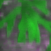
\includegraphics[width=\linewidth]{crop.png}
  \caption{crop patch}\label{fig:crop sample}
\endminipage\hfill
\minipage{0.32\textwidth}
  
\includegraphics[width=\linewidth]{weed.png}
  \caption{weed patch}\label{fig:weed sample}
\endminipage\hfill
\minipage{0.32\textwidth}%
  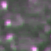
\includegraphics[width=\linewidth]{ground.png}
  \caption{ground patch}\label{fig:ground sample}
\endminipage
\end{figure}


\end{frame}

%------------------------------------------------

%------------------------------------------------
\section{Train the network}
%------------------------------------------------

\begin{frame}
\frametitle{MatConvNet}

To perform the given assignment I donloaded and installed MatConvNet library\footnote{http://www.vlfeat.org/matconvnet/}. Note that in order to use some functionalities of the library, such as using GPU acceleration, it has some requirements\footnote{http://www.vlfeat.org/matconvnet/gpu/}.
There is also a manual\footnote{http://www.vlfeat.org/matconvnet/matconvnet-manual.pdf} that explains all the blocks of a CNN both from the "mathematical" and "code function" view

\end{frame}

%------------------------------------------------

\begin{frame}
\frametitle{Example of CNN}
\begin{figure}[h]
	\begin{center}
		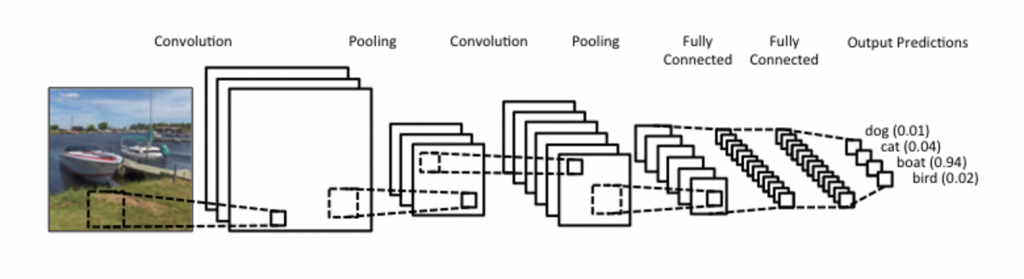
\includegraphics[scale=0.3]{CNN.png}
		\caption{Example of a Convolutional Neural Network}
		\label{fig:CNN}
	\end{center}
\end{figure}

\end{frame}

%------------------------------------------------

\begin{frame}
\frametitle{Block of a CNN}
The typical layers of a Convolutional Neural Network are:

\begin{itemize}

\item \textbf{Convolutional layer}

\item \textbf{Pooling Layer}

\item \textbf{Fully-connected layer}

\item \textbf{ReLu}

\item \textbf{SoftMax}

\end{itemize}

\end{frame}

%------------------------------------------------

\begin{frame}
\frametitle{Selected Architectures}

I selected different network architectures for comparing it, after the training, with the testing set. The architectures are:

\begin{enumerate}

\item $ INPUT \rightarrow [CONV \rightarrow RELU \rightarrow POOL]*2 \rightarrow FC \rightarrow RELU \rightarrow FC \rightarrow LOSS $ 

\item $ INPUT \rightarrow [CONV \rightarrow RELU \rightarrow POOL]*3 \rightarrow FC \rightarrow LOSS $ 

\item $ INPUT \rightarrow [CONV \rightarrow RELU \rightarrow POOL]*4 \rightarrow FC \rightarrow LOSS $ 

\item $ INPUT \rightarrow [CONV \rightarrow RELU \rightarrow POOL]*3 \rightarrow FC \rightarrow LOSS $ 

\item $ INPUT \rightarrow [CONV \rightarrow RELU \rightarrow POOL]*3 \rightarrow FC \rightarrow RELU \rightarrow FC \rightarrow LOSS $ 

\item $ INPUT \rightarrow [CONV \rightarrow RELU \rightarrow POOL]*3 \rightarrow [FC \rightarrow RELU]*2 \rightarrow FC \rightarrow LOSS $ 

\end{enumerate}

\end{frame}

%------------------------------------------------

\begin{frame}

\frametitle{Results of the training}
Here are the 6 network training graphs. On the left side there is the objective function and on the right side there is the error function.

\begin{figure}[h]
	\begin{center}
		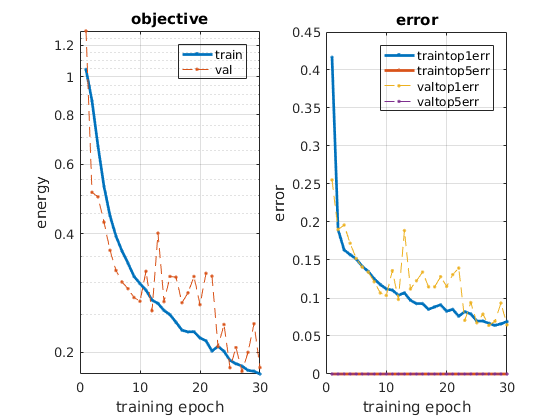
\includegraphics[scale=0.5]{init_1.png}
		\caption{network 1 training}
		\label{fig:training1}
	\end{center}
\end{figure}

\end{frame}

%------------------------------------------------

%------------------------------------------------

\begin{frame}

\begin{figure}[h]
	\begin{center}
		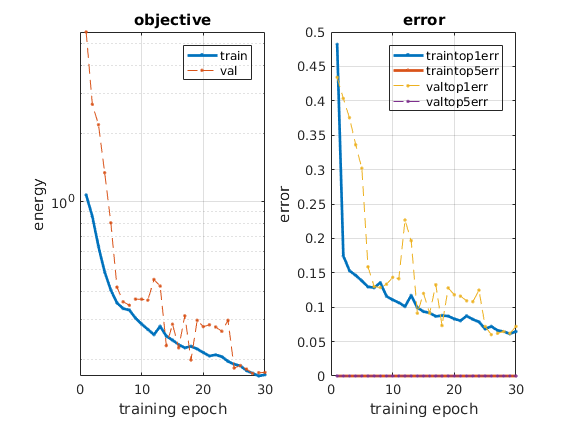
\includegraphics[scale=0.5]{init_2.png}
		\caption{network 2 training}
		\label{fig:training2}
	\end{center}
\end{figure}

\end{frame}

%------------------------------------------------


%------------------------------------------------

\begin{frame}


\begin{figure}[h]
	\begin{center}
		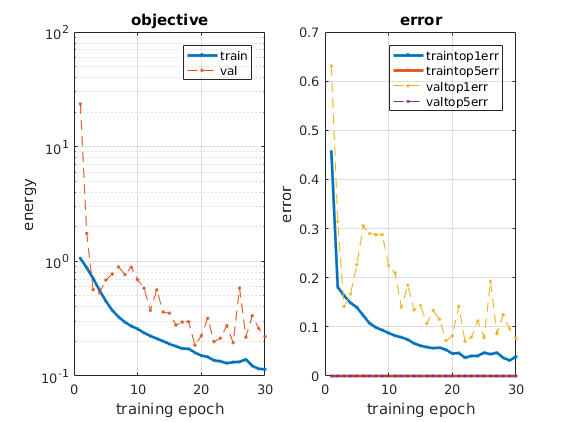
\includegraphics[scale=0.5]{init_3.png}
		\caption{network 3 training}
		\label{fig:training3}
	\end{center}
\end{figure}

\end{frame}

%------------------------------------------------


%------------------------------------------------

\begin{frame}


\begin{figure}[h]
	\begin{center}
		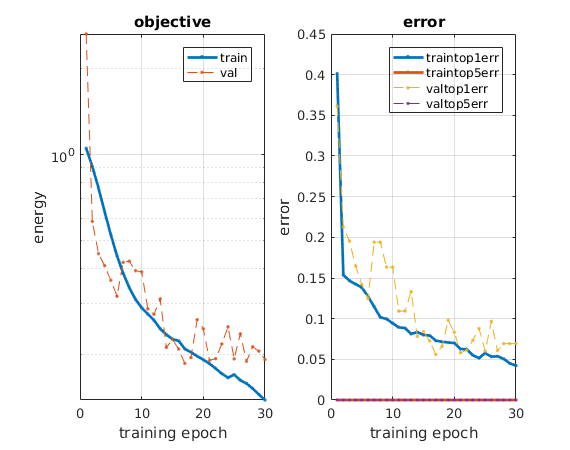
\includegraphics[scale=0.5]{init_4.png}
		\caption{network 4 training}
		\label{fig:training4}
	\end{center}
\end{figure}

\end{frame}

%------------------------------------------------


%------------------------------------------------

\begin{frame}


\begin{figure}[h]
	\begin{center}
		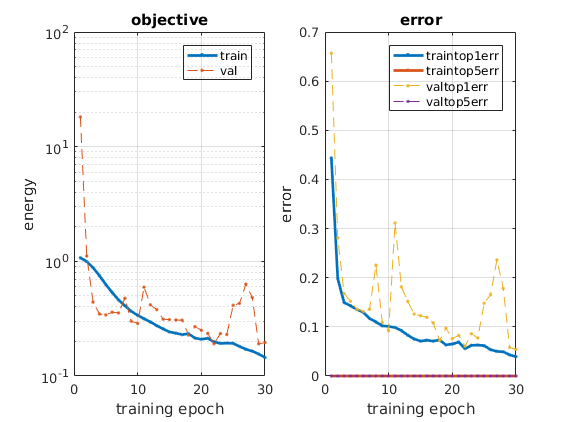
\includegraphics[scale=0.5]{init_5.png}
		\caption{network 5 training}
		\label{fig:training5}
	\end{center}
\end{figure}

\end{frame}

%------------------------------------------------


%------------------------------------------------

\begin{frame}


\begin{figure}[h]
	\begin{center}
		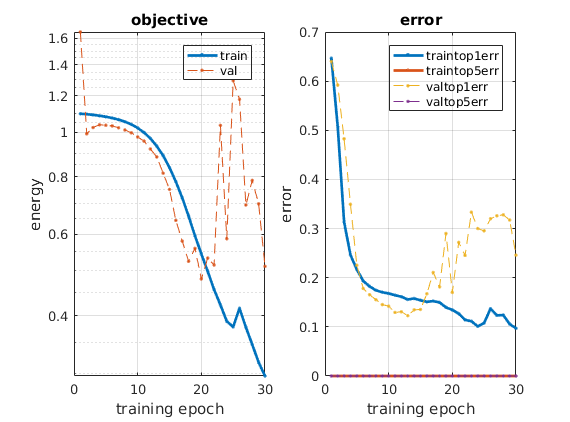
\includegraphics[scale=0.5]{init_6.png}
		\caption{network 6 training}
		\label{fig:training6}
	\end{center}
\end{figure}


\end{frame}

%------------------------------------------------

%------------------------------------------------
\section{Evaluate the network}
%------------------------------------------------

%------------------------------------------------


\begin{frame}
\frametitle{Accuracy}

In order to evaluate the network I calculated the accuracy. The accuracy can be computed as:

\begin{center}

	$ ACC= \frac{TP+TN}{TP+TN+FP+FN} $

\end{center}

where $ TP = $ true positive , $ TN =$ true negative , $ FP =$ false positive  and $ FN =$ false negative 

\end{frame}

%------------------------------------------------

%------------------------------------------------
\begin{frame}
\frametitle{Results of the six networks}

\begin{table}
\centering

\begin{tabular}{|c|c|c|c|c|}
 \hline
 \textbf{Network} & \textbf{Accuracy} & \textbf{Acc Crop} & \textbf{Acc Ground} & \textbf{Acc Weed} \\ \hline
 1 & 94,00\% & 92,80\%  & 99,80\%  & 89,40\%  \\ \hline
 2 & 94,07\% & 95,60\%  & 99,80\%  & 86,80\%  \\ \hline
 3 & 92,53\% & 92,20\%  & 99,80\%  & 85,60\%  \\ \hline
 4 & 94,13\% & 93,00\%  & 99,80\%  & 89,60\%  \\ \hline
 \textbf{5} & \textbf{94,20\%} & \textbf{94,00\%}  & \textbf{99,80\%}  & \textbf{88,80\%}  \\ \hline
 6 & 92,33\% & 93,60\%  & 99,80\%  & 83,60\%  \\ \hline
\end{tabular}
\end{table}

\end{frame}

\begin{frame}
\frametitle{Accuracy of network 5 with different configurations of number of maps of the filters}
\begin{table} [h]
\begin{center}
\begin{tabular}{|c|c|c|c|c|}
 \hline
 \textbf{Filter 1} & \textbf{Filter 2} & \textbf{Filter 3} & \textbf{Filter 4} & \textbf{Accuracy} \\ \hline
 10 & 20 & 40  & 80  & 94,20\%  \\ \hline
 15 & 30 & 60  & 120  & 92,60\%  \\ \hline
 \textbf{8} & \textbf{16} & \textbf{32}  & \textbf{64}  & \textbf{94,33\%}  \\ \hline
 7 & 14 & 28  & 56  & 93,73\%  \\ \hline
 9 & 18 & 36  & 72  & 93,20\%  \\ \hline
 12 & 24 & 48  & 96  & 92,53\%  \\ \hline
 
\end{tabular}
\end{center} 
\end{table}

\end{frame}

\begin{frame}
\frametitle{Confusion Matrix}

I calculated also the confusion matrix, also known as error matrix, that is a specific table layout that allows visualization of the performance of the classifier.

The Confusion matrix, for the testing set, is:

\begin{table}[h]
\centering

\begin{tabular}{cl|c|c|c|}
\cline{3-5}
\multicolumn{1}{l}{}                                         &        & \multicolumn{3}{c|}{\textbf{Predicted}}                                             \\ \cline{3-5} 
\textbf{}                                                    &        & \multicolumn{1}{l|}{crop} & \multicolumn{1}{l|}{weed} & \multicolumn{1}{l|}{ground} \\ \hline
\multicolumn{1}{|c|}{\multirow{3}{*}{\textbf{Actual Class}}} & crop   & 472                       & 28                        & 0                           \\ \cline{2-5} 
\multicolumn{1}{|c|}{}                                       & weed   & 55                        & 445                       & 0                           \\ \cline{2-5} 
\multicolumn{1}{|c|}{}                                       & ground & 1                         & 0                         & 499                         \\ \hline
\end{tabular}
\end{table} 

\end{frame}

\begin{frame}
\frametitle{Sliding Window approach}

\begin{itemize}

	\item take a testing image. The size of the testing image is $ 966\times 1296\times 3$
	\item extract patches from that.I used patches of size $ 51\times 51 \times 3 $. 				  I used two kind of stride: 10 and 15. So I obtained respectively $ 11500 $ and $ 		 		  5063 $ patches
	\item make a new image the same size of the original testing image. On this image, I 					  painted the central pixel of each of the patches with a color depending on the best  		  class that the classifier choosed. The color used are the same of the annotation 		          image of the dataset CWFID:green for crop, red for weed and black for ground
	\item repeat for all the images of the testing set

\end{itemize}

\end{frame}


\begin{frame}
\frametitle{Sliding Window Problem}

Here is an example of the result of the sliding window
\begin{figure}[!htb]
\minipage{0.5\textwidth}
  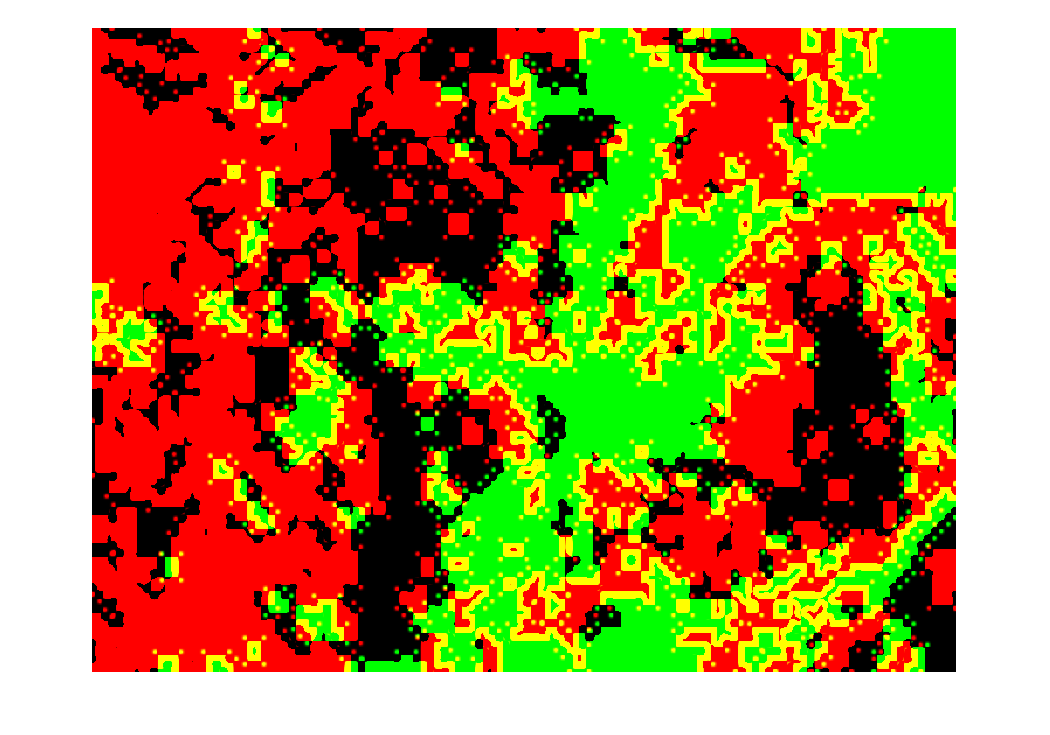
\includegraphics[width=\linewidth]{stride10im1.png}
  \caption{sliding window stride=10}\label{fig: sliding window problem}
\endminipage\hfill
\minipage{0.5\textwidth}
  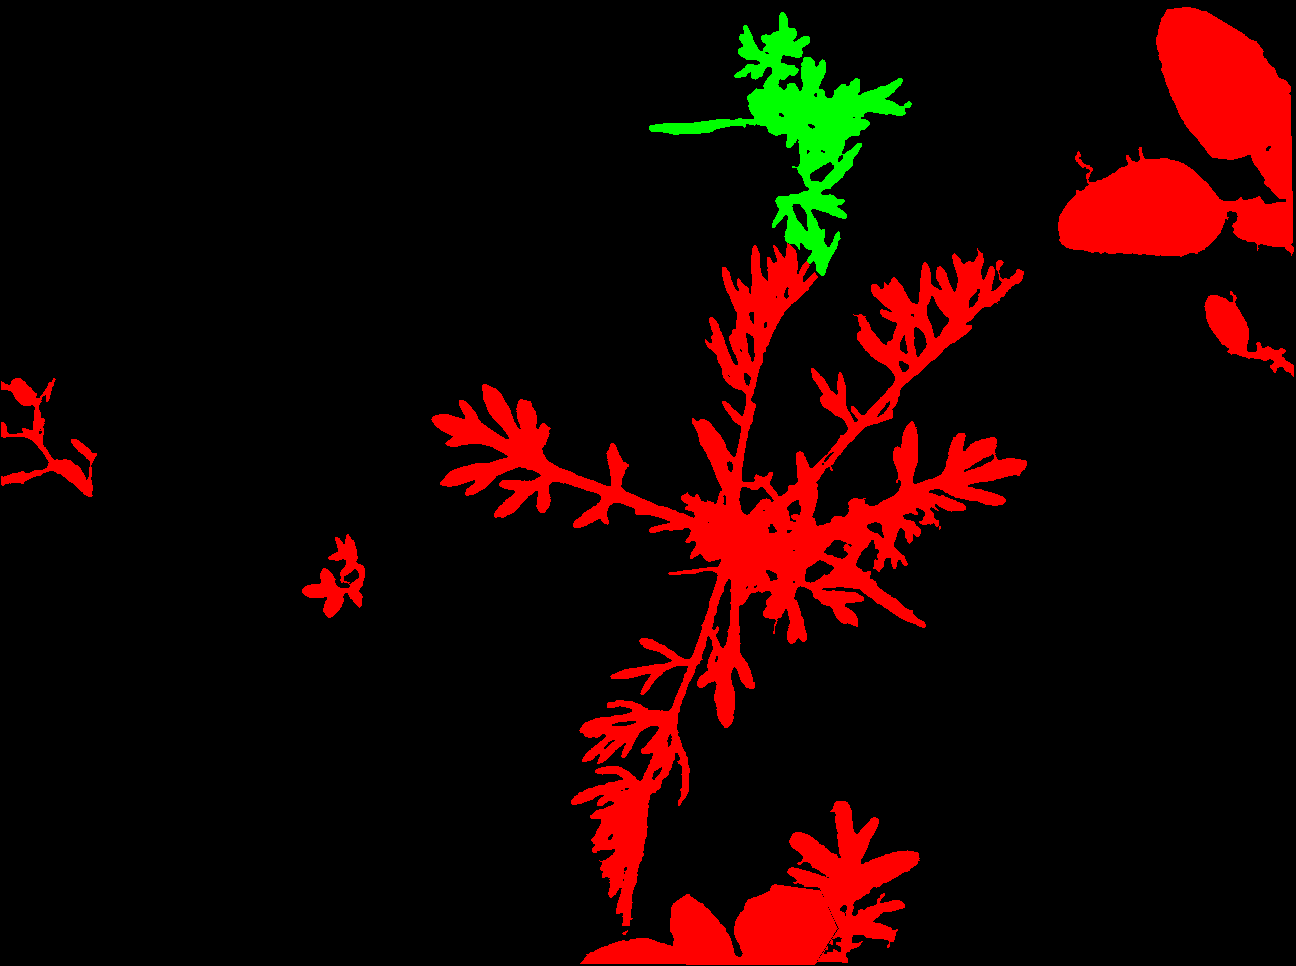
\includegraphics[width=\linewidth]{annotation.png}
  \caption{annotation}\label{fig:annotation}
\endminipage\hfill
\end{figure}
\newpage

\end{frame}

\begin{frame}
\frametitle{Umbalanced class problem}

The problem was that the network suffers of umbalanced data. Umbalanced data typically refers to a problem of classification where the classes are not represented equally.On the training set:

\begin{itemize}

	\item \textbf{92,50\%} of the pixels are marked as ground
	\item \textbf{5,96\%} of the pixels are marked as weed
	\item \textbf{1,54\%} of the pixels are marked as crop

\end{itemize}


\end{frame}

\begin{frame}
\frametitle{Using a Threshold for Ground}

 The threshold must be a value for which the 92,50\% of the ground probability are bigger.In other words:

\begin{center}
	$ T = groundVector[numberOfPatches\times 0,9250] $
\end{center}

where $groundVector $ is the vector containing the probabilities of the ground patches in descending order and $numberOfPatches $ is the number of patches apply to the image.

\end{frame}

\begin{frame}
\frametitle{Using a Threshold also for crop}
The results looks better with an accuracy close to $ 70\% $ but the networks failed to classify crop form weed.
Solution:
\begin{itemize}
	\item use a threshold also for crop
\end{itemize}

\end{frame}

\begin{frame}

\frametitle{Results}
The accuracy was 91,25\% for sliding window with stride 15 and 89,62\% for a stride of 10
\begin{figure}[h]
  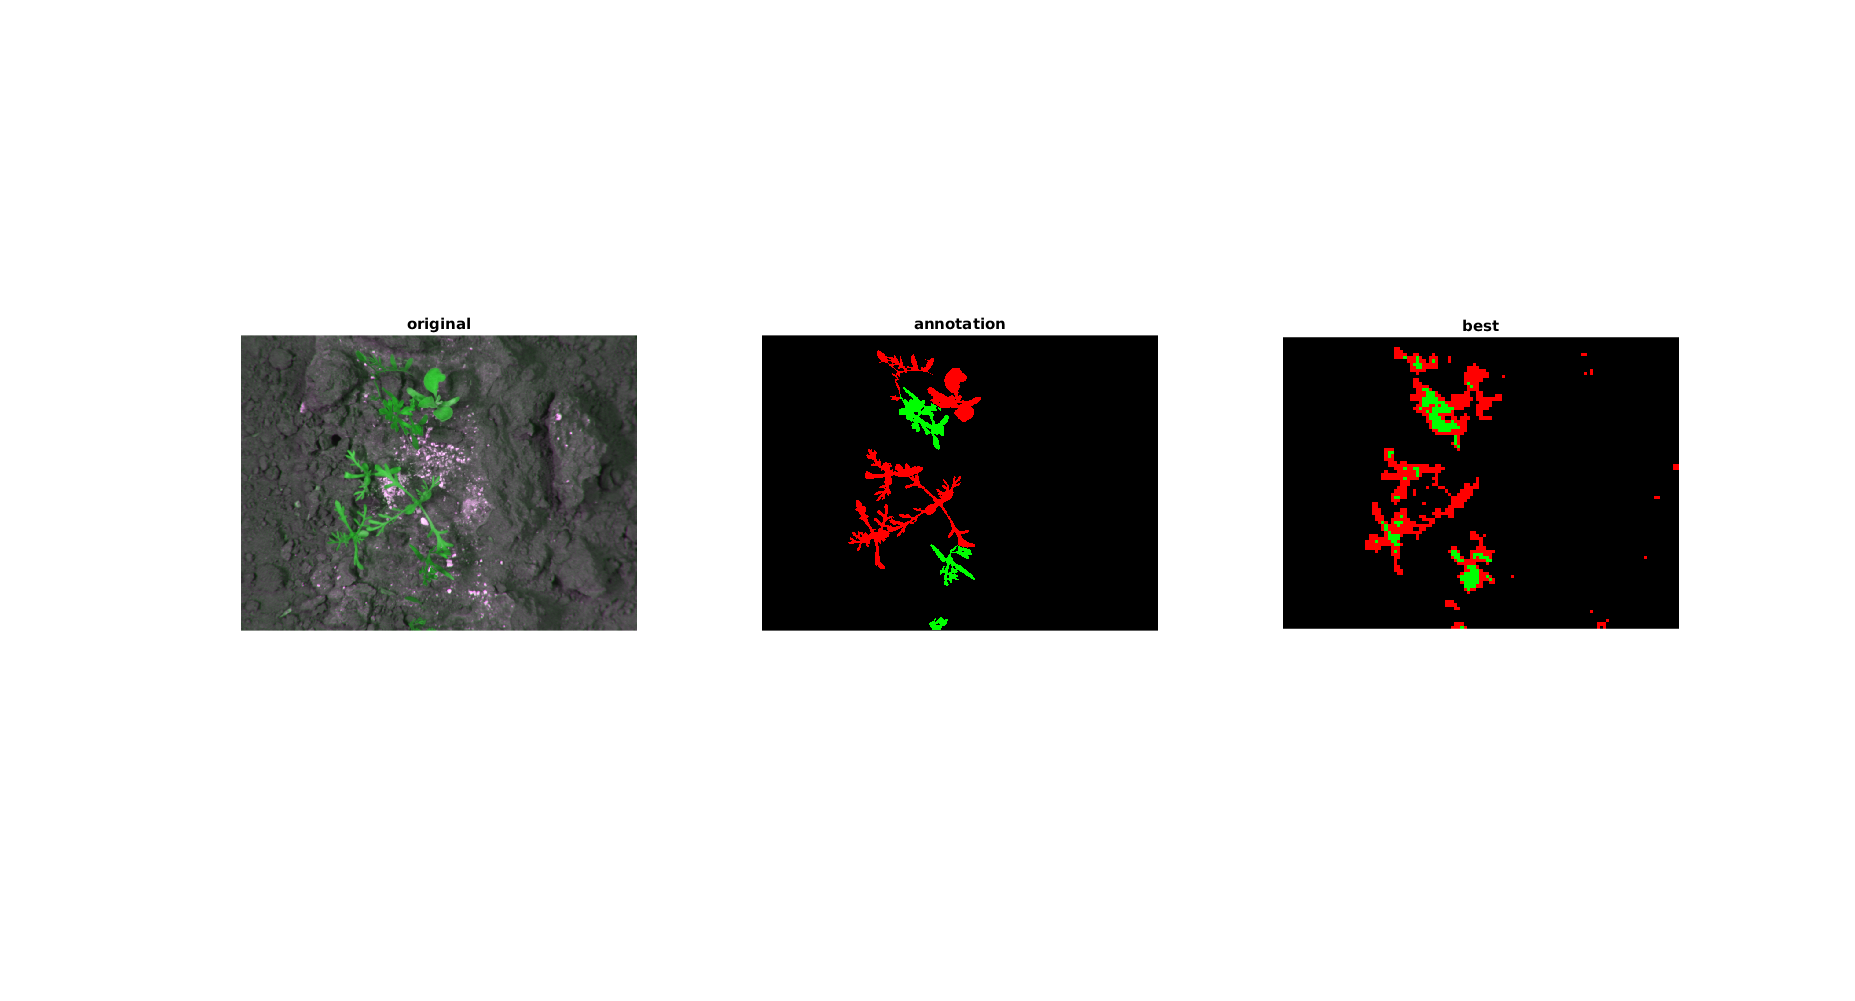
\includegraphics[width=\linewidth]{2.png}
  \caption{sliding window stride=10}\label{fig: sliding window 10 1}
\end{figure}
\end{frame}

%------------------------------------------------
\section{Summary and future extensions}
%------------------------------------------------

\begin{frame}
\frametitle{Network classifier problem}
The network fails when there are a lot of crop and weed with respect to the training set frequency percentage

\begin{figure}[h]
	\begin{center}
		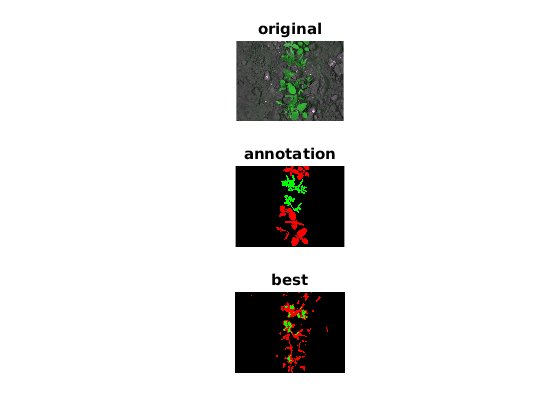
\includegraphics[width=\linewidth]{15.png}
		\caption{bad sliding window result}
		\label{fig:bad sliding window result}
	\end{center}
\end{figure}

\end{frame}

\begin{frame}
\frametitle{Possible solutions}
\begin{itemize}

	\item \textbf{have a larger dataset}: if we have more patches the network could possibly work 			          better. In order to have more patches rotation could be applied
	
	\item \textbf{resampling the dataset}: 
   \begin{enumerate}
   
		\item we can add copies of instances from the under-represented class called over-		              sampling,or more formally sampling with replacement
		\item we can delete instances from the over-represented class, called under-sampling
   
   \end{enumerate}
   
   \item \textbf{try penalized models}: we can use the same algorithms but give them a different perspective on the problem. 
Penalized classification imposes an additional cost on the model for making classification mistakes on the minority class during training. These penalties can bias the model to pay more attention to the minority class 
\end{itemize}
\end{frame}


\end{document}
              
            